\documentclass[../main.tex]{subfiles}
\begin{document}

\chapter{Basic principles for approximating differential equations}
	\label{chap:chap_11}
	%\pagenumbering{arabic}
	
	\noindent The finite element method is a very flexible approach for solving partial differential equations. Its two most attractive features are the ease of handling domains of complex shape in two and three dimensions and the ease of constructing higherorder discretization methods. The finite element method is usually applied for discretization in space, and therefore spatial problems will be our focus in the coming sections. Extensions to time-dependent problems may, for instance, use finite difference approximations in time.
	
	Before studying how finite element methods are used to tackle differential equation, we first look at how global basis functions and the least squares, Galerkin, and collocation principles can be used to solve differential equations.

\section[Differential equation models]{Differential equation models}
\label{sec:sec_11_1}
	Let us consider an abstract differential equation for a function $u(x)$ of one variable, written as
	
	\begin{equation}
		\label{eqa117}		
		\mathcal{L}(u)=0, \quad x \in \Omega .
	\end{equation}
	
	Here are a few examples on possible choices of $\mathcal{L}(u)$, of increasing complexity:
	
	\begin{equation}
		\label{eqa118}
		\mathcal{L}(u)=\frac{d^{2} u}{d x^{2}}-f(x) \\
	\end{equation}
	
	\begin{equation}
		\label{eqa119}
		\mathcal{L}(u)=\frac{d}{d x}\left(\alpha(x) \frac{d u}{d x}\right)+f(x) \\
	\end{equation}
	
	\begin{equation}
		\label{eqa120}
		\mathcal{L}(u)=\frac{d}{d x}\left(\alpha(u) \frac{d u}{d x}\right)-a u+f(x) \\
	\end{equation}
	
	\begin{equation}
		\label{eqa121}
		\mathcal{L}(u)=\frac{d}{d x}\left(\alpha(u) \frac{d u}{d x}\right)+f(u, x)
	\end{equation}
	
	\noindent Both $\alpha(x)$ and $f(x)$ are considered as specified functions, while $a$ is a prescribed parameter. Differential equations corresponding to (\ref{eqa118})-(\ref{eqa119}) arise in diffusion phenomena, such as steady transport of heat in solids and flow of viscous fluids between flat plates. The form (\ref{eqa120}) arises when transient diffusion or wave phenomenon are discretized in time by finite differences. The equation (\ref{eqa121}) appear in chemical models when diffusion of a substance is combined with chemical reactions. Also in biology, (\ref{eqa121}) plays an important role, both for spreading of species and in models involving generation and propagation of electrical signals.
	
	Let $\Omega=[0, L]$ be the domain in one space dimension. In addition to the differential equation, $u$ must fulfill boundary conditions at the boundaries of the domain, $x=0$ and $x=L$. When $\mathcal{L}$ contains up to second-order derivatives, as in the examples above, $m=1$, we need one boundary condition at each of the (two) boundary points, here abstractly specified as
	
	\begin{equation}
		\label{eqa122}
		\mathcal{B}_{0}(u)=0, x=0, \quad \mathcal{B}_{1}(u)=0, x=L
	\end{equation}
	
	\noindent There are three common choices of boundary conditions:
	
	\begin{equation}
		\label{eqa123}
		\mathcal{B}_{i}(u)  =u-g,  \text { Dirichlet condition } \\
	\end{equation}

	\begin{equation}
		\label{eqa124}
		\mathcal{B}_{i}(u)  =-\alpha \frac{d u}{d x}-g,  \text { Neumann condition } \\
	\end{equation}

	\begin{equation}
		\label{eqa125}
		\mathcal{B}_{i}(u) =-\alpha \frac{d u}{d x}-h(u-g),  \text { Robin condition }
	\end{equation}	

	\noindent Here, $g$ and $a$ are specified quantities.
	
	From now on we shall use $u_{e}(x)$ as symbol for the exact solution, fulfilling
	
	\begin{equation}
		\label{eqa126}
		\mathcal{L}\left(u_{\mathrm{e}}\right)=0, \quad x \in \Omega,
	\end{equation}
	
	\noindent while $u(x)$ is our notation for an approximate solution of the differential equation.
	
	\begin{mybox}
		\textbf{Remark on notation.}
		
		\noindent In the literature about the finite element method, is common to use $u$ as the exact solution and $u_{h}$ as the approximate solution, where $h$ is a discretization parameter. However, the vast part of the present text is about the approximate solutions, and having a subscript $h$ attached all the time is cumbersome. Of equal importance is the close correspondence between implementation and mathematics that we strive to achieve in this text: when it is natural to use \textbf{\texttt{u}} and not \textbf{\texttt{u\_h}} in code, we let the mathematical notation be dictated by the code's preferred notation. After all, it is the powerful computer implementations of the finite element method that justifies studying the mathematical formulation and aspects of the method.	
	\end{mybox}
	
	\section[Basic principles for approximating differential equations]{Simple model problems}
	\label{sec:sec_11_2}
	\noindent A common model problem used much in the forthcoming examples is
	
	\begin{equation}
		\label{eqa127}
		-u^{\prime \prime}(x)=f(x), \quad x \in \Omega=[0, L], \quad u(0)=0, u(L)=D .
	\end{equation}

	\noindent A closely related problem with a different boundary condition at $x=0$ reads
	
	\begin{equation}
		\label{eqa128}
		-u^{\prime \prime}(x)=f(x), \quad x \in \Omega=[0, L], \quad u^{\prime}(0)=C, u(L)=D .
	\end{equation}

	\noindent A third variant has a variable coefficient,
	
	\begin{equation}
		\label{eqa129}
		-\left(\alpha(x) u^{\prime}(x)\right)^{\prime}=f(x), \quad x \in \Omega=[0, L], \quad u^{\prime}(0)=C, u(L)=D .
	\end{equation}

	We can easily solve these using sympy. For (\ref{eqa127}) we can write the function
	
	\begin{lstlisting}[numbers=none]
		def model1(f, L, D):
		"""Solve -u'' = f(x), u(0)=0, u(L)=D."""
		u_x = - sp.integrate(f, (x, 0, x)) + c_0
		u = sp.integrate(u_x, (x, 0, x)) + c_1
		r = sp.solve([u.subs(x, 0)-0, u.subs(x,L)-D], [c_0, c_1])
		u = u.subs(c_0, r[c_0]).subs(c_1, r[c_1])
		u = sp.simplify(sp.expand(u))
		return u
	\end{lstlisting}
	
	\noindent Calling \textbf{model1(2, L, D)} results in the solution
	
	\begin{equation}
		\label{eqa130}
		u(x)=\frac{1}{L} x\left(D+L^{2}-L x\right)
	\end{equation}

	\noindent Model (\ref{eqa128}) can be solved by
	
	\begin{lstlisting}[numbers=none]
		def model2(f, L, C, D):
		"""Solve -u'' = f(x), u'(0)=C, u(L)=D."""
		u_x = - sp.integrate(f, (x, 0, x)) + c_0
		u = sp.integrate(u_x, (x, 0, x)) + c_1
		r = sp.solve([sp.diff(u,x).subs(x, 0)-C, u.subs(x,L)-D], [c_0, c_1])
		u = u.subs(c_0, r[c_0]).subs(c_1, r[c_1])
		u = sp.simplify(sp.expand(u))
		return u
	\end{lstlisting}
	
	\noindent to yield
	
	\begin{equation}
		\label{eqa131}
		u(x)=-x^{2}+C x-C L+D+L^{2},
	\end{equation}

	\noindent if $f(x)=2$. Model (\ref{eqa129}) requires a bit more involved code,
	
	
	\begin{lstlisting}[numbers=none]
		def model3(f, a, L, C, D):
		"""Solve -(a*u')' = f(x), u(0)=C, u(L)=D."""
		au_x = - sp.integrate(f, (x, 0, x)) + c_0
		u = sp.integrate(au_x/a, (x, 0, x)) + c_1
		r = sp.solve([u.subs(x, 0)-C, u.subs(x,L)-D], [c_0, c_1])
		u = u.subs(c_0, r[c_0]).subs(c_1, r[c_1])
		u = sp.simplify(sp.expand(u))
		return u
	\end{lstlisting}
	
	\noindent With $f(x)=0$ and $\alpha(x)=1+x^{2}$ we get
	
	$$u(x)=\frac{C \operatorname{atan}(L)-C \operatorname{atan}(x)+D \operatorname{atan}(x)}{\operatorname{atan}(L)}$$
	
\section[Forming the residual]{Forming the residual} 
	\label{sec:sec_11_3}
	\noindent The fundamental idea is to seek an approximate solution $u$ in some space $V$,

	$$
	V=\operatorname{span}\left\{\psi_{0}(x), \ldots, \psi_{N}(x)\right\},
	$$
	
	\noindent which means that $u$ can always be expressed as a linear combination of the basis functions $\left\{\varphi_{i}\right\}_{i \in \mathcal{I}_{s}}$, with $\mathcal{I}_{s}$ as the index set $\{0, \ldots, N\}$ :
	$$
	u(x)=\sum_{j \in \mathcal{I}_{s}} c_{j} \psi_{j}(x)
	$$
	The coefficients $\left\{c_{i}\right\}_{i \in \mathcal{I}_{s}}$ are unknowns to be computed.
	(Later, in Section 14, we will see that if we specify boundary values of $u$ different from zero, we must look for an approximate solution $u(x)=B(x)+$ $\sum_{j} c_{j} \psi_{j}(x)$, where $\sum_{j} c_{j} \psi_{j} \in V$ and $B(x)$ is some function for incorporating the right boundary values. Because of $B(x), u$ will not necessarily lie in $V$. This modification does not imply any difficulties.)
	
	We need principles for deriving $N+1$ equations to determine the $N+1$ unknowns $\left\{c_{i}\right\}_{i \in \mathcal{I}_{s}}$. When approximating a given function $f$ by $u=\sum_{j} c_{j} \varphi_{j}, \mathrm{a}$ key idea is to minimize the square norm of the approximation error $e=u-f$ or (equvalently) demand that $e$ is orthogonal to $V$. Working with $e$ is not so useful here since the approximation error in our case is $e=u_{e}-u$ and $u_{\mathrm{e}}$ is unknown. The only general indicator we have on the quality of the approximate solution is to what degree $u$ fulfills the differential equation. Inserting $u=\sum_{j} c_{j} \psi_{j}$ into $\mathcal{L}(u)$ reveals that the result is not zero, because $u$ is only likely to equal $u_{\mathrm{e}}$. The nonzero result,

	\begin{equation}
		\label{eqa132}
		R=\mathcal{L}(u)=\mathcal{L}\left(\sum_{j} c_{j} \psi_{j}\right),
	\end{equation}

	\noindent is called the residual and measures the error in fulfilling the governing equation.
	Various principles for determining $\left\{c_{i}\right\}_{i \in \mathcal{I}_{\text {s }}}$ try to minimize $R$ in some sense. Note that $R$ varies with $x$ and the $\left\{c_{i}\right\}_{i \in \mathcal{I}_{s}}$ parameters. We may write this dependence explicitly as
	
	\begin{equation}
		\label{eqa133}
		R=R\left(x ; c_{0}, \ldots, c_{N}\right)
	\end{equation}

	\noindent Below, we present three principles for making $R$ small: a least squares method, a projection or Galerkin method, and a collocation or interpolation method.
	
\section[The least squares method]{The least squares method} 
	\label{sec:sec_11_4}

	\noindent The least-squares method aims to find $\left\{c_{i}\right\}_{i \in \mathcal{I}_{s}}$ such that the square norm of the residual
	
	\begin{equation}
		\label{eqa134}
		\|R\|=(R, R)=\int_{\Omega} R^{2} \mathrm{~d} x
	\end{equation}

	\noindent is minimized. By introducing an inner product of two functions $f$ and $g$ on $\Omega$ as
	
	\begin{equation}
		\label{eqa135}
		(f, g)=\int_{\Omega} f(x) g(x) \mathrm{d} x,
	\end{equation}

	\noindent the least-squares method can be defined as
	
	\begin{equation}
		\label{eqa136}
	\min _{c_{0}, \ldots, c_{N}} E=(R, R) .
	\end{equation}

	\noindent Differentiating with respect to the free parameters $\left\{c_{i}\right\}_{i \in \mathcal{I}_{s}}$ gives the $N+1$ equations

	\begin{equation}
		\label{eqa137}
		\int_{\Omega} 2 R \frac{\partial R}{\partial c_{i}} \mathrm{~d} x=0 \quad \Leftrightarrow \quad\left(R, \frac{\partial R}{\partial c_{i}}\right)=0, \quad i \in \mathcal{I}_{s}
	\end{equation}

	\section[The Galerkin method]{The Galerkin method} 
	\label{sec:sec_11_5}
	
	\noindent The least-squares principle is equivalent to demanding the error to be orthogonal to the space $V$ when approximating a function $f$ by $u \in V$. With a differential equation we do not know the true error so we must instead require the residual $R$ to be orthogonal to $V$. This idea implies seeking $\left\{c_{i}\right\}_{i \in \mathcal{I}_{s}}$ such that
	
	\begin{equation}
		\label{eqa138}
		(R, v)=0, \quad \forall v \in V .
	\end{equation}

	\noindent This is the Galerkin method for differential equations.
	
	This statement is equivalent to $R$ being orthogonal to the $N+1$ basis functions only:

	\begin{equation}
		\label{eqa139}
		\left(R, \psi_{i}\right)=0, \quad i \in \mathcal{I}_{s},
	\end{equation}

	resulting in $N+1$ equations for determining $\left\{c_{i}\right\}_{i \in \mathcal{I}_{s}}$.

\section[Basic principles for approximating differential equations]{The Method of Weighted Residuals}
	\label{sec:sec_11_6} 
	\noindent A generalization of the Galerkin method is to demand that $R$ is orthogonal to some space $W$, but not necessarily the same space as $V$ where we seek the unknown function. This generalization is naturally called the \emph{method of weighted residuals}:

	\begin{equation}
		\label{eqa140}
		(R, v)=0, \quad \forall v \in W .
	\end{equation}
	
	\noindent If $\left\{w_{0}, \ldots, w_{N}\right\}$ is a basis for $W$, we can equivalently express the method of weighted residuals as
	
	\begin{equation}
		\label{eqa141}
		\left(R, w_{i}\right)=0, \quad i \in \mathcal{I}_{s} .
	\end{equation}

	\noindent The result is $N+1$ equations for $\left\{c_{i}\right\}_{i \in \mathcal{I}_{s}}$.

	The least-squares method can also be viewed as a weighted residual method with $w_{i}=\partial R / \partial c_{i}$.
	
	\begin{mybox}
		\textbf{Variational formulation of the continuous problem.}
		
		\noindent Formulations like (\ref{eqa140}) (or (\ref{eqa141})) and (\ref{eqa138}) (or (\ref{eqa139})) are known as \emph{variational formulations}. These equations are in this text primarily used for a numerical approximation $u \in V$, where $V$ is a \emph{finite-dimensional} space with dimension $N+1$. However, we may also let $V$ be an \emph{infinite-dimensional} space containing the exact solution $u_{e}(x)$ such that also $u_{e}$ fulfills the same variational formulation. The variational formulation is in that case a mathematical way of stating the problem and acts as alternative to the usual formulation of a differential equation with initial and/or boundary conditions.
	\end{mybox}
	
	
\section[Test and Trial Functions]{Test and Trial Functions} 
	\label{sec:sec_11_7}
	\noindent In the context of the Galerkin method and the method of weighted residuals it is common to use the name \emph{trial function} for the approximate $u=\sum_{j} c_{j} \psi_{j}$. The space containing the trial function is known as the trial space. The function $v$ entering the orthogonality requirement in the Galerkin method and the method of weighted residuals is called \emph{test function}, and so are the $\psi_{i}$ or $w_{i}$ functions that are used as weights in the inner products with the residual. The space where the test functions comes from is naturally called the \emph{test space}.
	
	We see that in the method of weighted residuals the test and trial spaces are different and so are the test and trial functions. In the Galerkin method the test and trial spaces are the same (so far).
	
	\begin{mybox}
		\textbf{Remark.}
		
		\noindent It may be subject to debate whether it is only the form of (\ref{eqa140}) or (\ref{eqa138}) after integration by parts, as explained in Section \ref{sec:sec_11_10}, that qualifies for the term variational formulation. The result after integration by parts is what is obtained after taking the \emph{first variation} of an optimization problem, see Section \ref{sec:sec_11_13} However, here we use variational formulation as a common term for formulations which, in contrast to the differential equation $R=0$, instead demand that an average of $R$ is zero: $(R, v)=0$ for all $v$ in some space.
	\end{mybox}
	
\section[The collocation]{The collocation} 
	\label{sec:sec_11_8}
	\noindent The idea of the collocation method is to demand that $R$ vanishes at $N+1$ selected points $x_{0}, \ldots, x_{N}$ in $\Omega$ :
	
	\begin{equation}
		\label{eqa142}
		R\left(x_{i} ; c_{0}, \ldots, c_{N}\right)=0, \quad i \in \mathcal{I}_{s} .
	\end{equation}

	\noindent The collocation method can also be viewed as a method of weighted residuals with Dirac delta functions as weighting functions. Let $\delta\left(x-x_{i}\right)$ be the Dirac delta function centered around $x=x_{i}$ with the properties that $\delta\left(x-x_{i}\right)=0$ for $x \neq x_{i}$ and
	
	\begin{equation}
		\label{eqa143}
		\int_{\Omega} f(x) \delta\left(x-x_{i}\right) \mathrm{d} x=f\left(x_{i}\right), \quad x_{i} \in \Omega
	\end{equation}

	\noindent Intuitively, we may think of $\delta\left(x-x_{i}\right)$ as a very peak-shaped function around $x=x_{i}$ with integral 1, roughly visualized in Figure \ref{fig:img_46} . Because of (\ref{eqa143}), we can let $w_{i}=\delta\left(x-x_{i}\right)$ be weighting functions in the method of weighted residuals, and (\ref{eqa141}) becomes equivalent to (\ref{eqa142}).
	
	\begin{figure}[H]
		\centering
		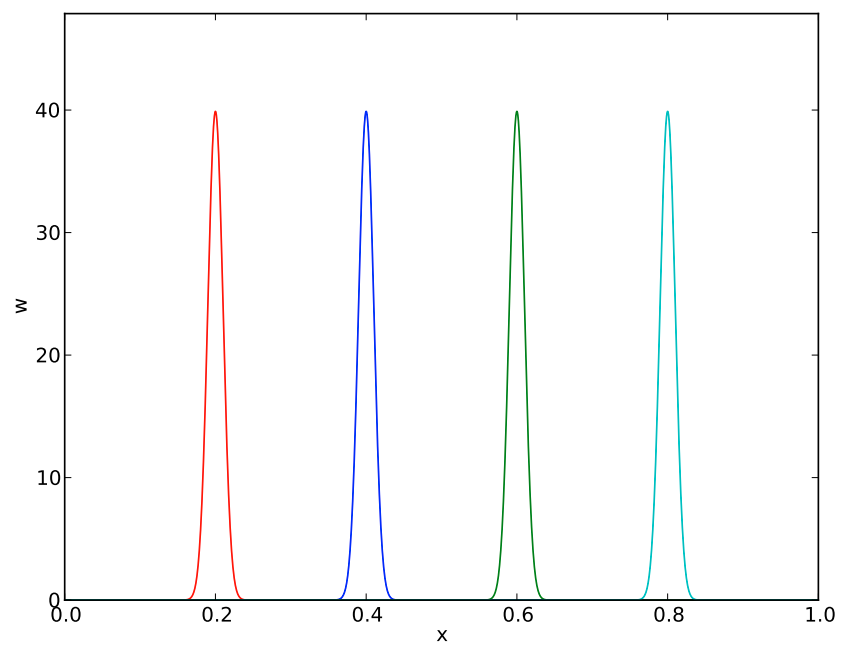
\includegraphics[width=0.7\linewidth]{img_46}
		\caption{Approximation of delta functions by narrow Gaussian functions.}
		\label{fig:img_46}
	\end{figure}
	
	\noindent \textbf{The subdomain collocation method.} The idea of this approach is to demand the integral of $R$ to vanish over $N+1$ subdomains $\Omega_{i}$ of $\Omega$ :
	
	\begin{equation}
		\label{eqa144}
		\int_{\Omega_{i}} R \mathrm{~d} x=0, \quad i \in \mathcal{I}_{s}
	\end{equation}

	\noindent This statement can also be expressed as a weighted residual method

	\begin{equation}
		\label{eqa145}
		\int_{\Omega} R w_{i} \mathrm{~d} x=0, \quad i \in \mathcal{I}_{s},
	\end{equation}

	\noindent where $w_{i}=1$ for $x \in \Omega_{i}$ and $w_{i}=0$ otherwise.

\section[Examples on using the principles]{Examples on using the principles} 
	\label{sec:sec_11_9}
	\noindent Let us now apply global basis functions to illustrate the principles for minimizing $R$.
	
	\noindent \textbf{The model problem.    } We consider the differential equation problem
	
	\begin{equation}
		\label{eqa146}
		-u^{\prime \prime}(x)=f(x), \quad x \in \Omega=[0, L], \quad u(0)=0, u(L)=0
	\end{equation}
	
	\noindent \textbf{Basis functions.   } Our choice of basis functions $\psi_{i}$ for $V$ is
	
	\begin{equation}
		\label{eqa147}
		\psi_{i}(x)=\sin \left((i+1) \pi \frac{x}{L}\right), \quad i \in \mathcal{I}_{s} .
	\end{equation}

	An important property of these functions is that $\psi_{i}(0)=\psi_{i}(L)=0$, which means that the boundary conditions on $u$ are fulfilled:
	
	$$ u(0)=\sum_{j} c_{j} \psi_{j}(0)=0, \quad u(L)=\sum_{j} c_{j} \psi_{j}(L)=0. $$
	
	\noindent Another nice property is that the chosen sine functions are orthogonal on $\Omega$ :
	
	\begin{equation}
		\label{eqa148}
		\int_{0}^{L} \sin \left((i+1) \pi \frac{x}{L}\right) \sin \left((j+1) \pi \frac{x}{L}\right) 	\mathrm{d} x= \begin{cases}\frac{1}{2} L & i=j \\ 0, & i \neq j\end{cases}
	\end{equation}

	\noindent provided $i$ and $j$ are integers.
	
	\noindent\textbf{The residual.   } We can readily calculate the following explicit expression for the residual:
	
	\begin{equation}
		\label{eqa149}
		R\left(x ; c_{0}, \ldots, c_{N}\right) =u^{\prime \prime}(x)+f(x), \\
		=\frac{d^{2}}{d x^{2}}\left(\sum_{j \in \mathcal{I}_{s}} c_{j} \psi_{j}(x)\right)+f(x), \\
		=\sum_{j \in \mathcal{I}_{s}} c_{j} \psi_{j}^{\prime \prime}(x)+f(x) .
	\end{equation}
	
	\noindent \textbf{The least squares method.   } The equations (\ref{eqa137}) in the least squares method require an expression for $\partial R / \partial c_{i}$. We have
	
	\begin{equation}
		\label{eqa150}
		\frac{\partial R}{\partial c_{i}}=\frac{\partial}{\partial c_{i}}\left(\sum_{j \in 	\mathcal{I}_{s}} c_{j} \psi_{j}^{\prime \prime}(x)+f(x)\right)=\sum_{j \in \mathcal{I}_{s}} \frac{\partial c_{j}}{\partial c_{i}} \psi_{j}^{\prime \prime}(x)=\psi_{i}^{\prime \prime}(x) .
	\end{equation}

	\noindent The governing equations for $\left\{c_{i}\right\}_{i \in \mathcal{I}_{s}}$ are then
	
	\begin{equation}
		\label{eqa151}
		\left(\sum_{j} c_{j} \psi_{j}^{\prime \prime}+f, \psi_{i}^{\prime \prime}\right)=0, \quad i \in \mathcal{I}_{s},
	\end{equation}
	
	\noindent which can be rearranged as
	
	\begin{equation}
		\label{eqa152}
		\sum_{j \in \mathcal{I}_{s}}\left(\psi_{i}^{\prime \prime}, \psi_{j}^{\prime \prime}\right) 	c_{j}=-\left(f, \psi_{i}^{\prime \prime}\right), \quad i \in \mathcal{I}_{s} .
	\end{equation}

	\noindent This is nothing but a linear system
	$$\sum_{j \in \mathcal{I}_{s}} A_{i, j} c_{j}=b_{i}, \quad i \in \mathcal{I}_{s},$$
	with
	
	\begin{equation}
		\label{eqa153}
		\begin{aligned}
			A_{i, j} &=\left(\psi_{i}^{\prime \prime}, \psi_{j}^{\prime \prime}\right) \\
			&=\pi^{4}(i+1)^{2}(j+1)^{2} L^{-4} \int_{0}^{L} \sin \left((i+1) \pi \frac{x}{L}\right) \sin \left((j+1) \pi \frac{x}{L}\right) \mathrm{d} x \\
			&= \begin{cases}\frac{1}{2} L^{-3} \pi^{4}(i+1)^{4} & i=j \\
				0, & i \neq j\end{cases} \\
		\end{aligned}
	\end{equation}

	\begin{equation}
		\label{eqa154}
		b_{i} =-\left(f, \psi_{i}^{\prime \prime}\right)=(i+1)^{2} \pi^{2} L^{-2} \int_{0}^{L} f(x) \sin \left((i+1) \pi \frac{x}{L}\right) \mathrm{d} x
	\end{equation}

	\noindent Since the coefficient matrix is diagonal we can easily solve for
	
	\begin{equation}
		\label{eqa155}
		c_{i}=\frac{2 L}{\pi^{2}(i+1)^{2}} \int_{0}^{L} f(x) \sin \left((i+1) \pi \frac{x}{L}\right) 	\mathrm{d} x .
	\end{equation}

	\noindent With the special choice of $f(x)=2$ can be calculated in \textbf{\texttt{sympy}} by
	
	\begin{lstlisting}[numbers=none]
		from sympy import *
		import sys
		i, j = symbols('i j', integer=True)
		x, L = symbols('x L')
		f = 2
		a = 2*L/(pi**2*(i+1)**2)
		c_i = a*integrate(f*sin((i+1)*pi*x/L), (x, 0, L))
		c_i = simplify(c_i)
		print c_i
	\end{lstlisting}
	
	\noindent The answer becomes
	$$ c_{i}=4 \frac{L^{2}\left((-1)^{i}+1\right)}{\pi^{3}\left(i^{3}+3 i^{2}+3 i+1\right)}$$
	
	\noindent Now, $1+(-1)^{i}=0$ for $i$ odd, so only the coefficients with even index are nonzero. Introducing $i=2 k$ for $k=0, \ldots, N / 2$ to count the relevant indices (for $N$ odd, $k$ goes to $(N-1) / 2)$, we get the solution 

	\begin{equation}
		\label{eqa156}
		u(x)=\sum_{k=0}^{N / 2} \frac{8 L^{2}}{\pi^{3}(2 k+1)^{3}} \sin \left((2 k+1) \pi 	\frac{x}{L}\right)
	\end{equation}

	\noindent The coefficients decay very fast: $c_{2}=c_{0} / 27, c_{4}=c_{0} / 125$. The solution will therefore be dominated by the first term,

	$$ u(x) \approx \frac{8 L^{2}}{\pi^{3}} \sin \left(\pi \frac{x}{L}\right) $$

	\noindent\textbf{The Galerkin method.   } The Galerkin principle (\ref{eqa138}) applied to (\ref{eqa146}) consists of inserting our special residual (\ref{eqa149}) in (\ref{eqa138})

	$$ \left(u^{\prime \prime}+f, v\right)=0, \quad \forall v \in V, $$
	
	\noindent or
	
	\begin{equation}
		\label{eqa157}
		\left(u^{\prime \prime}, v\right)=-(f, v), \quad \forall v \in V .
	\end{equation}\

	\noindent This is the variational formulation, based on the Galerkin principle, of our differential equation. The $\forall v \in V$ requirement is equivalent to demanding the equation $\left(u^{\prime \prime}, v\right)=-(f, v)$ to be fulfilled for all basis functions $v=\psi_{i}, i \in \mathcal{I}_{s}$, see (\ref{eqa138}) and (\ref{eqa139}). We therefore have
	
	\begin{equation}
		\label{eqa158}
		\left(\sum_{j \in \mathcal{I}_{s}} c_{j} \psi_{j}^{\prime \prime}, \psi_{i}\right)=-\left(f, \psi_{i}\right), \quad i \in \mathcal{I}_{s} .
	\end{equation}

	\noindent This equation can be rearranged to a form that explicitly shows that we get a linear system for the unknowns $\left\{c_{i}\right\}_{i \in \mathcal{I}_{s}}$ :

	\begin{equation}
		\label{eqa159}
		\sum_{j \in \mathcal{I}_{s}}\left(\psi_{i}, \psi_{j}^{\prime \prime}\right) c_{j}=\left(f, 	\psi_{i}\right), \quad i \in \mathcal{I}_{s} .
	\end{equation}
	
	\noindent For the particular choice of the basis functions (\ref{eqa147}) we get in fact the same linear system as in the least squares method because $\psi^{\prime \prime}=-(i+1)^{2} \pi^{2} L^{-2} \psi$.\bigbreak
	
	\noindent \textbf{The collocation method.   } For the collocation method (\ref{eqa142}) we need to decide upon a set of $N+1$ collocation points in $\Omega$. A simple choice is to use uniformly spaced points: $x_{i}=i \Delta x$, where $\Delta x=L / N$ in our case $(N \geq 1)$. However, these points lead to at least two rows in the matrix consisting of zeros (since $\psi_{i}\left(x_{0}\right)=0$ and $\psi_{i}\left(x_{N}\right)=0$ ), thereby making the matrix singular and non-invertible. This forces us to choose some other collocation points, e.g., random points or points uniformly distributed in the interior of $\Omega$. Demanding the residual to vanish at these points leads, in our model problem (\ref{eqa146}), to the equations
		
	\begin{equation}
		\label{eqa160}
		-\sum_{j \in \mathcal{I}_{s}} c_{j} \psi_{j}^{\prime \prime}\left(x_{i}\right)=f\left(x_{i}\right), \quad i \in \mathcal{I}_{s},
	\end{equation}

	\noindent which is seen to be a linear system with entries
	$$ A_{i, j}=-\psi_{j}^{\prime \prime}\left(x_{i}\right)=(j+1)^{2} \pi^{2} L^{-2} \sin \left((j+1) \pi \frac{x_{i}}{L}\right) $$
	in the coefficient matrix and entries $b_{i}=2$ for the right-hand side (when $f(x)=2)$.
	
	The special case of $N=0$ can sometimes be of interest. A natural choice is then the midpoint $x_{0}=L / 2$ of the domain, resulting in $A_{0,0}=-\psi_{0}^{\prime \prime}\left(x_{0}\right)=\pi^{2} L^{-2}$, $f\left(x_{0}\right)=2$, and hence $c_{0}=2 L^{2} / \pi^{2} .$ \bigbreak
	
	\noindent \textbf{Comparison.} In the present model problem, with $f(x)=2$, the exact solution is $u(x)=x(L-x)$, while for $N=0$ the Galerkin and least squares method result in $u(x)=8 L^{2} \pi^{-3} \sin (\pi x / L)$ and the collocation method leads to $u(x)=$ $2 L^{2} \pi^{-2} \sin (\pi x / L)$. Since all methods fulfill the boundary conditions $u(0)=$ $u(L)=0$, we expect the largest discrepancy to occur at the midpoint of the domain: $x=L / 2$. The error at the midpoint becomes $-0.008 L^{2}$ for the Galerkin and least squares method, and $0.047 L^{2}$ for the collocation method. \bigbreak 

\section[Integration by parts]{Integration by parts} 
	\label{sec:sec_11_10}
	\noindent A problem arises if we want to apply popular finite element functions to solve our model problem (\ref{eqa146}) by the standard least squares, Galerkin, or collocation methods: the piecewise polynomials $\psi_{i}(x)$ have discontinuous derivatives at the cell boundaries which makes it problematic to compute the second-order derivative. This fact actually makes the least squares and collocation methods less suitable for finite element approximation of the unknown function. (By rewriting the equation $-u^{\prime \prime}=f$ as a system of two first-order equations, $u^{\prime}=v$ and $-v^{\prime}=$ $f$, the least squares method can be applied. Also, differentiating discontinuous functions can actually be handled by distribution theory in mathematics.) The Galerkin method and the method of weighted residuals can, however, be applied together with finite element basis functions if we use \emph{integration by parts} as a means for transforming a second-order derivative to a first-order one.
	
	Consider the model problem (\ref{eqa146}) and its Galerkin formulation
	$$ -\left(u^{\prime \prime}, v\right)=(f, v) \quad \forall v \in V . $$
	
	\noindent Using integration by parts in the Galerkin method, we can move a derivative of $u$ onto $v$ :
	
	\begin{equation}
		\label{eqa161}
		\int_{0}^{L} u^{\prime \prime}(x) v(x) \mathrm{d} x =-\int_{0}^{L} u^{\prime}(x) v^{\prime}(x) \mathrm{d} x+\left[v u^{\prime}\right]_{0}^{L} \\
		=-\int_{0}^{L} u^{\prime}(x) v^{\prime}(x) \mathrm{d} x+u^{\prime}(L) v(L)-u^{\prime}(0) v(0) .
	\end{equation}
	
	\noindent Usually, one integrates the problem at the stage where the $u$ and $v$ functions enter the formulation. Alternatively, but less common, we can integrate by parts in the expressions for the matrix entries:
	=
	\begin{equation}
		\label{eqa162}
		\int_{0}^{L} \psi_{i}(x) \psi_{j}^{\prime \prime}(x) \mathrm{d} x =-\int_{0}^{L} \psi_{i}^{\prime}(x) \psi_{j}^{\prime}(x) d x+\left[\psi_{i} \psi_{j}^{\prime}\right]_{0}^{L} \\
		=-\int_{0}^{L} \psi_{i}^{\prime}(x) \psi_{j}^{\prime}(x) \mathrm{d} x+\psi_{i}(L) \psi_{j}^{\prime}(L)-\psi_{i}(0) \psi_{j}^{\prime}(0) .
	\end{equation}

	\noindent Integration by parts serves to reduce the order of the derivatives and to make the coefficient matrix symmetric since $\left(\psi_{i}^{\prime}, \psi_{j}^{\prime}\right)=\left(\psi_{i}^{\prime}, \psi_{j}^{\prime}\right)$. The symmetry property depends on the type of terms that enter the differential equation. As will be seen later in Section \ref{chap:chap_15}, integration by parts also provides a method for implementing boundary conditions involving $u^{\prime}$.
	
	With the choice (\ref{eqa147}) of basis functions we see that the "boundary terms" $\psi_{i}(L) \psi_{j}^{\prime}(L)$ and $\psi_{i}(0) \psi_{j}^{\prime}(0)$ vanish since $\psi_{i}(0)=\psi_{i}(L)=0$.
	
	\noindent \textbf{Weak form.   } Since the variational formulation after integration by parts make weaker demands on the differentiability of $u$ and the basis functions $\psi_{i}$, the resulting integral formulation is referred to as a \emph{weak form} of the differential equation problem. The original variational formulation with second-order derivatives, or the differential equation problem with second-order derivative, is then the \emph{strong form}, with stronger requirements on the differentiability of the functions.
	
	For differential equations with second-order derivatives, expressed as variational formulations and solved by finite element methods, we will always perform integration by parts to arrive at expressions involving only first-order derivatives.

\section[Boundary function]{Boundary function} 
	\label{sec:sec_11_11}
	\noindent So far we have assumed zero Dirichlet boundary conditions, typically $u(0)=$ $u(L)=0$, and we have demanded that $\psi_{r}(0)=\psi_{i}(L)=0$ for $i \in \mathcal{I}_{s}$. What about a boundary condition like $u(L)=D \neq 0$ ? This condition immediately faces a problem: $u=\sum_{j} c_{j} \varphi_{j}(L)=0$ since all $\varphi_{i}(L)=0$.
	
	A boundary condition of the form $u(L)=D$ can be implemented by demanding that all $\psi_{n}(L)=0$, but adding a boundary function $B(x)$ with the right boundary value, $B(L)=D$, to the expansion for $u$ :
	
	$$
	u(x)=B(x)+\sum_{j \in \mathcal{I}_{s}} c_{j} \psi_{j}(x) .
	$$
	This $u$ gets the right value at $x=L$ :
	$$
	u(L)=B(L)+\sum_{j \in I_{a}} c_{j} \psi_{j}(L)=B(L)=D .
	$$
	The idea is that for any boundary where $u$ is known we demand $\psi_{y}$ to vanish and construct a function $B(x)$ to attain the boundary value of $u$. There are no restrictions how $B(x)$ varies with $x$ in the interior of the domain, so this variation needs to be constructed in some way.
	
	For example, with $u(0)=0$ and $u(L)=D$, we can choose $B(x)=x D / L$, since this form ensures that $B(x)$ fulfills the boundary conditions: $B(0)=0$ and $B(L)=D$. The unknown function is then sought on the form
	
	\begin{equation}
	\label{eqa163}
		u(x)=\frac{x}{L} D+\sum_{j \in \mathcal{I}_{*}} c_{j} \psi_{j}(x)
	\end{equation}

	\noindent with $\psi_{i}(0)=\psi_{1}(L)=0$. 
	
	The $B(x)$ function can be chosen in many ways as long as its boundary values are correct. For example, $B(x)=D(x / L)^{p}$ for any power $p$ will work fine in the above example.
	
	As another example, consider a domain $\Omega=[a, b]$ where the boundary conditions are $u(a)=U_{a}$ and $u(b)=U_{b}$. A class of possible $B(x)$ functions is
	
	\begin{equation}
	\label{eqa164}
		B(x)=U_{a}+\frac{U_{b}-U_{a}}{(b-a)^{\mathrm{p}}}(x-a)^{\mathrm{p}}, \quad p>0 .
	\end{equation}

	\noindent Real applications will most likely use the simplest version, $p=1$, but here such a $p$ parameter was included to demonstrate the ambiguity in the construction of $B(x)$.
	
	\begin{mybox}
		\textbf{Summary.}
		
		\noindent The general procedure of incorporating Dirichlet boundary conditions goes as follows. Let $O \Omega_{E}$ be the part(s) of the boundary OS of the domain $\Omega$ where $u$ is specified. Set $\psi_{u}=0$ at the points in OOR and seek $u$ as
		
		\begin{equation}
		\label{eqa165}
			u(x)=B(x)+\sum_{j \in \mathcal{I}_{s}} c_{y} \psi_{j}(x)
		\end{equation}
			
		where $B(x)$ equals the boundary conditions on $u$ at $\partial \Omega_{E}$.
	\end{mybox}
	

	\noindent \textbf{Remark.   } With the $B(x)$ term, $u$ does not in general lie in $V=\operatorname{span}\left\{\psi_{0}, \ldots, \psi_{N}\right\}$ anymore. Moreover, when a prescribed value of $u$ at the boundary, say u( $a)=U_{a}$ is different from zero, it does not make sense to say that $u$ lies in a vector space, because this space does not obey the requirements of addition and scalar multiplication. For example, $2 u$ does not lie in the space since its boundary value is $2 U_{a}$, which is incorrect. It only makes sense to split $u$ in two parts, as done above, and have the unknown part $\sum_{j} c_{j} \psi_{j}$ in a proper function space.

\section[Abstract notatiom for variational formulations]{Abstract notatiom for variational formulations} 
	\label{sec:sec_11_12}
	\noindent We have seen that variational formulations end up with a formula involving $u$ and $v$, such as $\left(u^{\prime}, v^{\prime}\right)$ and a formula involving $v$ and known functions, such as $(f, v)$. A widely used notation is to introduce an abstract variational statement written as $a(u, v)=L(v)$, where $a(u, v)$ is a so-called \emph{bilinear} form involving all the terms that contain both the test and trial function, while $L(v)$ is a \emph{linear} form containing all the terms without the trial function. For example, the statement
	$$
	\int_{\Omega} u^{\prime} v^{\prime} \mathrm{d} x=\int_{\Omega} f v \mathrm{~d} x \quad \text { or } \quad\left(u^{\prime}, v^{\prime}\right)=(f, v) \quad \forall v \in V
	$$
	can be written in abstract form: find $u$ such that
	$$
	a(u, v)=L(v) \quad \forall v \in V
	$$
	where we have the definitions
	$$
	a(u, v)=\left(u^{\prime}, v^{\prime}\right), \quad L(v)=(f, v) \text {. }
	$$
	
	The term \emph{linear} means that $L\left(\alpha_{1} v_{1}+\alpha_{2} v_{2}\right)=\alpha_{1} L\left(v_{1}\right)+\alpha_{2} L\left(v_{2}\right)$ for two test functions $v_{1}$ and $v_{2}$, and scalar parameters $\alpha_{1}$ and $\alpha_{2}$. Similarly, the term \emph{bilinear} means that $a(u, v)$ is linear in both its arguments:
	$$
	\begin{aligned}
		&a\left(\alpha_{1} u_{1}+\alpha_{2} u_{2}, v\right)=\alpha_{1} a\left(u_{1}, v\right)+\alpha_{2} a\left(u_{2}, v\right) \\
		&a\left(u, \alpha_{1} v_{1}+\alpha_{2} v_{2}\right)=\alpha_{1} a\left(u, v_{1}\right)+\alpha_{2} a\left(u, v_{2}\right)
	\end{aligned}
	$$
	In nonlinear problems these linearity properties do not hold in general and the abstract notation is then $F(u ; v)=0$.
	
	The matrix system associated with $a(u, v)=L(v)$ can also be written in an abstract form by inserting $v=\psi_{i}$ and $u=\sum_{j} c_{j} \psi_{j}$ in $a(u, v)=L(v)$. Using the linear properties, we get
	$$
	\sum_{j \in \mathcal{I}_{s}} a\left(\psi_{j}, \psi_{i}\right) c_{j}=L\left(\psi_{i}\right), \quad i \in \mathcal{I}_{s}
	$$
	which is a linear system
	$$
	\sum_{j \in \mathcal{I}_{s}} A_{i, j} c_{j}=b_{i}, \quad i \in \mathcal{I}_{s}
	$$
	where
	$$
	A_{i, j}=a\left(\psi_{j}, \psi_{i}\right), \quad b_{i}=L\left(\psi_{i}\right)
	$$
	
	\noindent In many problems, $a(u, v)$ is symmetric such that $a\left(\psi_{j}, \psi_{i}\right)=a\left(\psi_{i}, \psi_{j}\right)$. In those cases the coefficient matrix becomes symmetric, $A_{i, j}=A_{j, i}$, a property that can simplify solution algorithms for linear systems and make them more stable in addition to saving memory and computations.
	
	The abstract notation $a(u, v)=L(v)$ for linear differential equation problems is much used in the literature and in description of finite element software (in particular the FEniCS documentation). We shall frequently summarize variational forms using this notation.
	
\section[Basic principles for approximating differential equations]{Variational problems and optimization} 
	\label{sec:sec_11_13}
	
	
	\noindent If $a(u, v)=a(v, u)$, it can be shown that the variational statement
	$$
	a(u, v)=L(v) \quad \forall v \in V,
	$$
	is equivalent to minimizing the functional
	$$
	F(v)=\frac{1}{2} a(v, v)-L(v)
	$$
	over all functions $v \in V$. That is,
	$$
	F(u) \leq F(v) \quad \forall v \in V .
	$$
	Inserting a $v=\sum_{j} c_{j} \psi_{j}$ turns minimization of $F(v)$ into minimization of a quadratic function
	$$
	\bar{F}\left(c_{0}, \ldots, c_{N}\right)=\sum_{j \in \mathcal{I}_{s}} \sum_{i \in \mathcal{I}_{\bar{s}}} a\left(\psi_{i}, \psi_{j}\right) c_{i} c_{j}-\sum_{j \in \mathcal{I}_{s}} L\left(\psi_{j}\right) c_{j}
	$$
	of $N+1$ parameters.
	Minimization of $\bar{F}$ implies
	$$
	\frac{\partial \bar{F}}{\partial c_{i}}=0, \quad i \in \mathcal{I}_{s} .
	$$
	After some algebra one finds
	$$
	\sum j \in \mathcal{I}_{s} a\left(\psi_{i}, \psi_{j}\right) c_{j}=L\left(\psi_{i}\right), \quad i \in \mathcal{I}_{s}
	$$
	which is the same system as that arising from $a(u, v)=L(v)$.\bigbreak 
	Many traditional applications of the finite element method, especially in solid mechanics and structural analysis, start with formulating $F(v)$ from physical principles, such as minimization of energy, and then proceeds with deriving $a(u, v)=L(v)$, which is the equation usually desired in implementations.

	
\clearpage
\end{document} 
